
\subsection{Analytical solution}

Before going into the properties and the analytical solution to certain
boundary--value problems related to the diagonal flow case, a question that
arises naturally is the following: why shall we bother about the properties of a
problem analytically when we can solve it numerically? There exists two reasons:
\begin{itemize}
	\item The properties of a certain partial differential equation dictate what
	computational methods are suitable to solve it. For instance, consider
	\begin{equation} \label{eq:heat_problem_example}
		\begin{aligned}
			\left\{
				\begin{aligned}
					u_t - u_{xx} &= 0 & &\text{in } \real \times (0,\infty) \\
					u &= g & &\text{on } \real \times \{ t = 0 \}
				\end{aligned}
			\right.
		\end{aligned}
	\end{equation}
	\begin{equation} \label{eq:wave_problem_example}
		\begin{aligned}
			\left\{
				\begin{aligned}
					u_{tt} - u_{xx} &= 0 & &\text{in } \real \times \real \\
					u &= d & &\text{on } \real \times \{ t = 0 \} \\
					u_t &= h & &\text{on } \real \times \{ t = 0 \}
				\end{aligned}
			\right.
		\end{aligned}
	\end{equation}
	where $g, d, h \colon \real \to \real$ are given functions and $u = u(x,t)$
	is the unknown. Problems \eqref{eq:heat_problem_example} and
	\eqref{eq:wave_problem_example} are the typical diffusion problem and wave
	equation problem on the real line. If $g$ is a continuous function, it is
	widely known that the solution to \eqref{eq:heat_problem_example} is a
	$\mathcal{C}^\infty(\real \times (0,\infty))$, but in general it is only
	defined for positive times. Therefore the diffusion equation has a
	regularizing effect on the initial condition $g$. Now assume $d \in
	\mathcal{C}^2(\real)$ and $h \in \mathcal{C}^1(\real)$. Then the solution to
	\eqref{eq:wave_problem_example} is a $\mathcal{C}^2(\real \times \real)$,
	hence the wave equation does no make the initial conditions smoother, but is
	defined both for positive and negative times. Intuitively, the enormous
	differences between the properties of problems
	\eqref{eq:heat_problem_example} and \eqref{eq:wave_problem_example} should
	warn that different numerical methods should be used to solve them.
	
	\item Boundary--value problems and initial--value problems which are not
	well--posed might have more than one solution in a certain sense that must
	be specified. Hence if a problem with no unique solution is solved
	numerically, it is uncertain what solution is obtained and whether it has
	physical meaning.
\end{itemize}

As we have previously seen, Péclet's number is defined as
\begin{equation*}
	\peclet = 
	\frac{\text{convection transport rate}}{\text{diffusion transport rate}} = 
	\frac{\rho v_0 L}{\Gamma}
\end{equation*}
Note that the factor $\beta$ in the PDE from problem
\eqref{eq:diagonal_case_cauchy_problem} is a constant determined by the
geometry, whereas Peclet's number depends on the fluid and on the velocity
field. Since no more factors intervene on the PDE, this tells us that the
behaviour of the solution will depend greatly on Peclet's number. 

\subsubsection{Classical solution for \texorpdfstring{$\peclet =
\infty$}{infinite Péclet's number}}

Whenever $\peclet \to +\infty$, it implies $\Gamma \to 0^+$ since infinite
values for the density, velocity or characteristic length make no physical
sense. Therefore the difussion coefficient tends to $0$, which means the
Laplacian term, linked to the diffusion process, is negligible. Dividing the PDE
from \eqref{eq:diagonal_case_cauchy_problem} by Péclet's number results in the
following equation
\begin{equation} \label{eq:diagonal_case_cauchy_problem_infinite_peclet_eq1}
	\phi_x + \phi_y = 0 \quad \text{in } \Omega
\end{equation}
The following natural step would be considering equation
\eqref{eq:diagonal_case_cauchy_problem_infinite_peclet_eq1} with $g$ as boundary
condition on all $\partial \Omega$, that is to say, the following problem:
\begin{equation} \label{eq:diagonal_case_cauchy_problem_infinite_peclet_overdetermined_problem}
	\left\{
	\begin{aligned}
		\phi_x + \phi_y &= 0 &
		&\text{in } \Omega \\
		\phi &= g &
		&\text{on } \partial \Omega
	\end{aligned}
	\right.
\end{equation}
Nonetheless, problem
\eqref{eq:diagonal_case_cauchy_problem_infinite_peclet_overdetermined_problem}
is ``overdetermined'', which means a part of the boundary condition is
unnecessary due to the geometric properties of the PDE as we shall see. In order
to obtain a problem we can solve, take the curve $C = \left( [0,L] \times \{ 0
\} \right) \cup \left( \{ 0 \} \times (0,L] \right)$, and let $\tilde{g} \colon
C \subset \real^2 \rightarrow \real$ be
\begin{equation*}
	\tilde{g}(x,y) = 
	\left\{
	\begin{aligned}
		&\phi_\text{low} 	& &\text{if } (x,y) \in [0,L] \times \{ 0 \} \\
		&\phi_\text{high} 	& &\text{if } (x,y) \in \{ 0 \} \times (0,L] \\
	\end{aligned}
	\right.
\end{equation*}
which is the restriction of $g$ to $C$, that is to say, $\tilde{g} = g
\rvert_C$. The resulting Cauchy problem is
\begin{equation} \label{eq:diagonal_case_cauchy_problem_infinite_peclet}
	\left\{
	\begin{aligned}
		\phi_x + \phi_y &= 0 &
		&\text{in } \Omega \\
		\phi &= \tilde{g} &
		&\text{on } C
	\end{aligned}
	\right.
\end{equation}
The PDE from \eqref{eq:diagonal_case_cauchy_problem_infinite_peclet} is known as
the transport equation, which is a first--order linear PDE. In our case it has
constant coefficients, making it easier to solve analitically.\footnote{Actually
equation \eqref{eq:diagonal_case_cauchy_problem_infinite_peclet} is not the
transport equation, since neither $x$ nor $y$ are time variables but space
variables. The homogeneous transport equation is $u_t + b \vdot \grad{u} = 0$ in
$\real^n \times (0,\infty)$ where $u \colon \real^n \times [0,\infty) \to \real$
is the unknown. The importance of the time variable is that it gives the
``cylinder'' $\real^n \times [0,\infty) \subset \real^{n+1}$ where the equation
occurs. Nonetheless problem
\eqref{eq:diagonal_case_cauchy_problem_infinite_peclet} takes place in the
domain $(0, L) \times (0, L)$ which is a cylinder as well, hence the $y$
variable can be regarded as a time variable and solve the equation.}

\begin{definition*}
	A classical solution to problem
	\eqref{eq:diagonal_case_cauchy_problem_infinite_peclet} is a function $\phi
	\colon \overline{\Omega} \rightarrow \real$ such that:
	\begin{enumerate}[label={(\roman*)}, topsep=0pt]
		\item $\phi \in \mathcal{C}^1(\overline{\Omega})$, \ie $\phi$ is a
		$\mathcal{C}^1(\Omega)$ function that admits a $\mathcal{C}^1$ extension
		to an open neighbourhood of every point in $\partial \Omega$,
		\item $\phi$ satisfies the PDE and
		\item $\phi$ satisfies the boundary conditions.
	\end{enumerate}
\end{definition*}
\noindent
In order to find the solution to
\eqref{eq:diagonal_case_cauchy_problem_infinite_peclet}, we will assume $\phi$
is a $\mathcal{C}^1(\overline{\Omega})$ function. Once we find the solution we
will be able to tell whether $\phi$ is a classical solution. Moreover, so as to
find a candidate of solution, we will make some assumptions motivated by
intuiton and with lack of rigour, and later we shall justify them properly. This
is a common practice in PDE theory.

We introduce some notation that will be useful. Given $m$ vectors $\vb{w}_1,
\ldots, \vb{w}_m \in \real^n$, the set $[\vb{w}_1, \ldots, \vb{w}_m] = \{
\sum_{i=1}^m \lambda_i \vb{w}_i \mid \lambda_1, \ldots, \lambda_m \in \real \}$
is the vector subspace of $\real^n$ spanned by $\vb{w}_1, \ldots, \vb{w}_m$. If
$W \subset \real^m$ is a vector subspace, $W^\perp = \{ v \in \real^n \mid v
\vdot w = 0 \ \forall w \in W \}$ is the vector subspace orthogonal to $W$.

The method we will follow to find the solution is known as the method of
characteristics. Using $\grad{\phi}$ we can write the PDE as
\begin{equation} \label{eq:diagonal_case_cauchy_problem_infinite_peclet_orthogonal_vectors}
	\left( 1, 1 \right)
	\vdot
	\grad{\phi}(x,y) = 
	\left( 1, 1 \right)
	\vdot
	\begin{pmatrix}
		\phi_x(x,y) \\ \phi_y(x,y)
	\end{pmatrix} = 
	\phi_x(x,y) + \phi_y(x,y) = 0
\end{equation}
Recall from vector calculus that the gradient vector of $\phi$ gives the
direction of maximum growth of $\phi$ at each point, whilst a non--zero vector
$\vb{w} \in [\grad{\phi}(x,y)]^\perp$ provides the direction at $(x,y)$ along
which $\phi$ remains constant. Equation
\eqref{eq:diagonal_case_cauchy_problem_infinite_peclet_orthogonal_vectors} tells
us that at each point $(x,y) \in \Omega$, $\phi$ is constant along the direction
given by $(1, 1)$. To prove this, we exploit the fact that the PDE is
first--order linear and use the chain rule to rewrite
\eqref{eq:diagonal_case_cauchy_problem_infinite_peclet_orthogonal_vectors}.
Consider a $\mathcal{C}^1$ mapping $\alpha(s) = (\alpha_1(s), \alpha_2(s))$ such
that $\alpha_1' = \alpha_2' = 1$ for all $s$. Since $\alpha$ is a mapping from
some subset of $\real$ to $\real^2$, its image
\begin{equation*}
	A = 
	\image \alpha = 
	\left\{ (x,y) \in \real^2 \mid x = \alpha_1(s), \ y = \alpha_2(s), \ s \in \real \right\}
\end{equation*}
can be thought of as a $\mathcal{C}^1$ curve. Moreover, we may choose the curve to
pass through $\Omega \cup C$ as we shall see in a moment. The restriction of $\phi$
to $A$, given by the composition $\varphi = \phi \circ \alpha \colon I \subset
\real \rightarrow \real$, is also a $\mathcal{C}^1$ function as it is
composition of $\mathcal{C}^1$ functions. By the chain rule,
\begin{equation} \label{eq:diagonal_case_cauchy_problem_infinite_peclet_chain_rule}
	\frac{\dd}{\dd{s}} \varphi(s) = 
	\frac{\dd}{\dd{s}} \phi(\alpha_1(s), \alpha_2(s)) = 
	\phi_x (\alpha_1(s), \alpha_2(s)) \alpha_1'(s) +  	
	\phi_y (\alpha_1(s), \alpha_2(s)) \alpha_2'(s) =
	\phi_x + \phi_y = 0
\end{equation}
where the last equality holds whenever $\alpha(s) \in \Omega$. Equation
\eqref{eq:diagonal_case_cauchy_problem_infinite_peclet_chain_rule} implies that
$\phi$ is constant on every connected component of $A \cap
\Omega$, thereby proving our claim. 

The following step is to find the curve $A$. Consider the mapping 
\begin{equation*}
	\begin{aligned}
		f \colon \real^3 &\longrightarrow \real^2 \\
		(s,x,y) &\longmapsto f(s,x,y) = (1,1)
	\end{aligned}
\end{equation*}
By taking a point $(x_0, y_0) \in \Omega \cup C$, we can find the curve $A$
passing by $(x_0, y_0)$:
\begin{equation} \label{eq:diagonal_case_cauchy_problem_infinite_peclet_characteristics_problem}
	\left\{
		\begin{aligned}
			&\alpha' = f(s,\alpha) = (1,1) & &\text{in } I \subset \real \\
			&\alpha(0) = (x_0, y_0)
		\end{aligned}
	\right.
\end{equation}
The function $f$ is constant, therefore is Lipschitz continuous on $(x,y)$ and
uniformly with respect to $s$, thus the solution to
\eqref{eq:diagonal_case_cauchy_problem_infinite_peclet_characteristics_problem}
exists and is unique due to the Picard--Lindelöf Theorem (Theorem
\ref{teo:picard_lindelof}). In addition, it is given by
\begin{equation} \label{eq:diagonal_case_cauchy_problem_infinite_peclet_characteristics_solution}
	\alpha(s) = (x_0 + s, y_0 + s) = (x_0, y_0) + s(1, 1) \quad s \in I \subset \real
\end{equation}
whence $A$ is the line passing by $(x_0, y_0)$ with director subspace $[(1,
1)]$. Moreover $A$ is not a single line, but rather a family of lines with
different initial condition. Hereinafter, we will take $(x_0,y_0) \in
C$\footnote{At the points $(x_0,y_0) \in C$ we have the boundary condition, \ie
we have information about the solution $\phi$.}. To distinguish the solutions
\eqref{eq:diagonal_case_cauchy_problem_infinite_peclet_characteristics_problem}
we will denote them by $\alpha(s; x_0, y_0)$, and the curves by $A_{(x_0,y_0)}$.

\begin{figure}[ht]
	\centering
	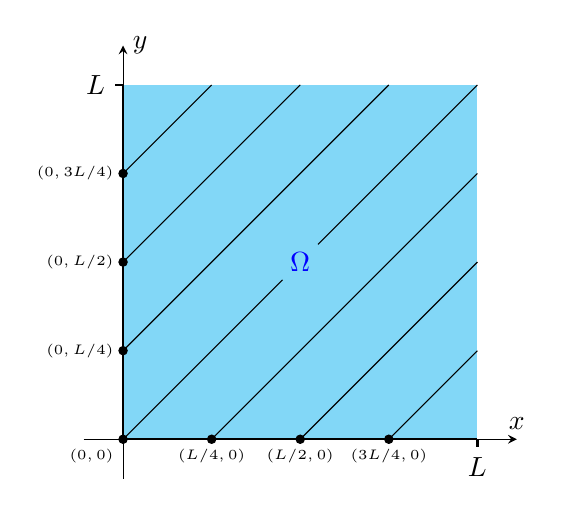
\begin{tikzpicture}
		% Lenghts
		\def\alength{5}
		\def\L{4.5}
		\def\mlength{0.1}
		% Axis
		\draw[-stealth] (0,-0.5) -- (0,\alength) node[right]{$y$};
		\draw[-stealth] (-0.5,0) -- (\alength,0) node[above]{$x$};
		\draw[black, thick] (\L,0) -- ++(0,-\mlength) node[below]{$L$};
		\draw[black, thick] (0,\L) -- ++(-\mlength,0) node[left]{$L$};
		% Domain
		\fill[cyan!70!white,opacity=0.7] (0,0) rectangle (\L, \L);
		\draw[thick, thick] (0,\L) -- (0,0) -- (\L,0);
		% Characteristics
%		\draw[black] (0,0) -- node[midway, above, rotate=45]{\tiny{$x - y = 0$}} (\L, \L);
		\node[blue] at ({0.5*\L}, {0.5*\L}) {$\Omega$};
		\draw[black] (0,0) -- ({0.45*\L}, {0.45*\L});
		\draw[black] ({0.55*\L}, {0.55*\L}) -- (\L, \L);		
		\draw[black] ({0.25*\L}, 0) -- (\L, {0.75*\L});
		\draw[black] ({0.50*\L}, 0) -- (\L, {0.50*\L});
		\draw[black] ({0.75*\L}, 0) -- (\L, {0.25*\L});		
		\draw[black] (0, {0.25*\L}) -- ({0.75*\L}, \L);
		\draw[black] (0, {0.50*\L}) -- ({0.50*\L}, \L);
		\draw[black] (0, {0.75*\L}) -- ({0.25*\L}, \L);
		% Points
		\filldraw[black] (0,{0.75*\L}) circle (1.5pt);
		\filldraw[black] (0,{0.50*\L}) circle (1.5pt);
		\filldraw[black] (0,{0.25*\L}) circle (1.5pt);
		\filldraw[black] (0,0) circle (1.5pt);
		\filldraw[black] ({0.25*\L},0) circle (1.5pt);
		\filldraw[black] ({0.50*\L},0) circle (1.5pt);
		\filldraw[black] ({0.75*\L},0) circle (1.5pt);
		% Text
		\node[black, anchor=east] at (0,{0.75*\L}) {\tiny{$(0,3L/4)$}};
		\node[black, anchor=east] at (0,{0.50*\L}) {\tiny{$(0,L/2)$}};
		\node[black, anchor=east] at (0,{0.25*\L}) {\tiny{$(0,L/4)$}};
		\node[black, anchor=north east] at (0,0) {\tiny{$(0,0)$}};
		\node[black, anchor=north] at ({0.25*\L},0) {\tiny{$(L/4,0)$}};
		\node[black, anchor=north] at ({0.50*\L},0) {\tiny{$(L/2,0)$}};
		\node[black, anchor=north] at ({0.75*\L},0) {\tiny{$(3L/4,0)$}};
	\end{tikzpicture}
	\captionsetup{width=0.70\linewidth}
	\caption{Some of the lines given by
	\eqref{eq:diagonal_case_cauchy_problem_infinite_peclet_characteristics_solution}
	with initial condition $(x_0,y_0) \in C$ extended to the top and right
	boundaries of $\Omega$.}
	\label{fig:diagonal_case_cauchy_problem_infinite_peclet_lines_from_C}
\end{figure}

We claim that a solution
\eqref{eq:diagonal_case_cauchy_problem_infinite_peclet_characteristics_solution}
can be extended so that $\alpha(s;x_0,y_0)$ eventually reaches the top or right
boundaries of $\Omega$ as shown in figure
\ref{fig:diagonal_case_cauchy_problem_infinite_peclet_lines_from_C}. Take $T >
0$ and $\delta > 0$ to be some constants to be determined and let $V = [0, T]
\times \overline{B((x_0,y_0), \delta)} \subset \real^3$. Since $f$ is a constant
function, we have
\begin{equation*}
	M = 
	\sup_{(s,x,y) \in V} \norm{f(s,x,y)} = 
	\max_{(s,x,y) \in V} \norm{f(s,x,y)} = 
	\sqrt{2}
\end{equation*} 
Again, by the Picard--Lindelöf theorem, the solution
\eqref{eq:diagonal_case_cauchy_problem_infinite_peclet_characteristics_solution}
exists for $s \in I = [0, T_0] \subset \real$ and remains in
$\overline{B((x_0,y_0), \delta)}$ where $T_0 = \min{\left\{ T, \frac{\delta}{M}
\right\}}$. By taking $\delta = \sqrt{2} L$ and $T = L$, applying the theorem we
obtain $T_0 = L$ and the solution stays in $\overline{B((x_0,y_0), \sqrt{2}
L)}$. Since $\sqrt{2} L$ is the maximum of the distances between two points
belonging to $\overline{\Omega}$, we have proved our claim. As a consequence, by
changing $(x_0,y_0)$ we can fill $\overline{\Omega}$ with these curves. All
except one of the solutions $\alpha(s;x_0,y_0)$ actually exit
$\overline{\Omega}$, however we do not care about the part of the curve outside
$\overline{\Omega}$\footnote{We have such freedom to choose the constants $T$
and $\delta$ because $f$ is a constant function.}.

Up to now, we have found out the following:
\begin{enumerate}[label={(\roman*)}, topsep=0pt]
	\item The lines given by $\alpha(s;x_0,y_0)$ can be extended so that both
	ends touch $\partial \Omega$. The implicit form of these is
	\begin{equation} \label{eq:diagonal_case_cauchy_problem_infinite_peclet_characteristics_implicit_form}
		A_{(x_0,y_0)} \colon x - y = x_0 - y_0, \quad (x_0,y_0) \in C
	\end{equation}
	\item The lines
	\eqref{eq:diagonal_case_cauchy_problem_infinite_peclet_characteristics_implicit_form}
	fill $\overline{\Omega}$.
	\item By equation
	\eqref{eq:diagonal_case_cauchy_problem_infinite_peclet_chain_rule}, the
	function $\phi$ is constant on every line
	\eqref{eq:diagonal_case_cauchy_problem_infinite_peclet_characteristics_implicit_form}.
	\label{eq:infinite_peclet_point_2}
\end{enumerate}
The curves
\eqref{eq:diagonal_case_cauchy_problem_infinite_peclet_characteristics_implicit_form}
are known as the characteristic lines (or simply characteristics) of problem
\eqref{eq:diagonal_case_cauchy_problem_infinite_peclet}. Some of them are
picture in figure
\ref{fig:diagonal_case_cauchy_problem_infinite_peclet_characteristics_problem}.

\begin{figure}[ht]
	\centering
	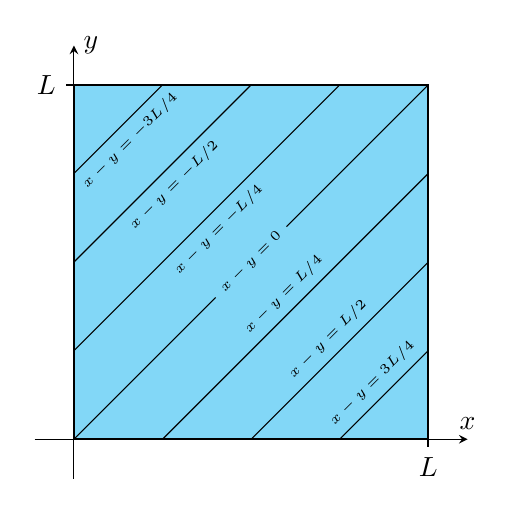
\begin{tikzpicture}
		% Lenghts
		\def\alength{5}
		\def\L{4.5}
		\def\mlength{0.1}
		% Axis
		\draw[-stealth] (0,-0.5) -- (0,\alength) node[right]{$y$};
		\draw[-stealth] (-0.5,0) -- (\alength,0) node[above]{$x$};
		\draw[black, thick] (\L,0) -- ++(0,-\mlength) node[below]{$L$};
		\draw[black, thick] (0,\L) -- ++(-\mlength,0) node[left]{$L$};
		% Domain
		\fill[cyan!70!white,opacity=0.7] (0,0) rectangle (\L, \L);
		\draw[thick, thick] (0,0) rectangle (\L, \L);
		% Characteristics
%		\draw[black] (0,0) -- node[midway, above, rotate=45]{\tiny{$x - y = 0$}} (\L, \L);
		\node[rotate=45] at ({0.5*\L}, {0.5*\L}) {\tiny{$x - y = 0$}};
		\draw[black] (0,0) -- ({0.4*\L}, {0.4*\L});
		\draw[black] ({0.6*\L}, {0.6*\L}) -- (\L, \L);
		
		\draw[black] ({0.25*\L}, 0) -- node[midway, above, rotate=45]{\tiny{$x - y = L/4$}} 
		(\L, {0.75*\L});
		\draw[black] ({0.50*\L}, 0) -- node[midway, above, rotate=45]{\tiny{$x - y = L/2$}} 
		(\L, {0.50*\L});
		\draw[black] ({0.75*\L}, 0) -- node[midway, above, rotate=45]{\tiny{$x - y = 3L/4$}} 
		(\L, {0.25*\L});
		
		
		
		\draw[black] (0, {0.25*\L}) -- node[midway, below, rotate=45]{\tiny{$x - y = -L/4$}} 
		({0.75*\L}, \L);
		\draw[black] (0, {0.50*\L}) -- node[midway, below, rotate=45]{\tiny{$x - y = -L/2$}} 
		({0.50*\L}, \L);
		\draw[black] (0, {0.75*\L}) -- node[midway, below, rotate=45]{\tiny{$x - y = -3L/4$}} 
		({0.25*\L}, \L);
	\end{tikzpicture}
	\caption{Some characteristics of problem \eqref{eq:diagonal_case_cauchy_problem_infinite_peclet}.}
	\label{fig:diagonal_case_cauchy_problem_infinite_peclet_characteristics_problem}
\end{figure}

We know the value of $\phi$ at $(x_0,y_0) \in C$ and $\phi$ is constant along
the curve $A_{(x_0,y_0)}$. Therefore the value of $\phi$ at $(x,y) \in
A_{(x_0,y_0)}$ is $\phi(x,y) = \phi(x_0,y_0) = \tilde{g}(x_0,y_0)$. As
$(x_0,y_0) \in C$ implies either $x_0 = 0$ or $y_0 = 0$ (or both), we have the following:
\begin{itemize}[topsep=0pt]
	\item If $y \leq x$ then $\phi(x,y) = \phi(x-y,0) = \tilde{g}(x-y,0)$.
	\item If $y > x$ then $\phi(x,y) = \phi(0,y-x) = \tilde{g}(0,y-x)$.
\end{itemize}
With this in mind, the solution to \eqref{eq:diagonal_case_cauchy_problem_infinite_peclet} is:
\begin{equation} \label{eq:diag_inf_pe_solution}
	\phi(x,y) = 
	\left\{
		\begin{aligned}
			&\tilde{g}(x-y,0) = \phi_\text{low} & &\text{if } y \leq x \\
			&\tilde{g}(0,y-x) = \phi_\text{high} & &\text{if } y > x \\
		\end{aligned}
	\right.
	\quad
	(x,y) \in \overline{\Omega}
\end{equation}
Intuitively, the characteristics give the paths in $\real^2$ through which the
information of the boundary conditions is transported. 

After finding the solution, we should check if $\phi \in
\mathcal{C}^1(\overline{\Omega})$. First consider the case when $\phi_\text{low}
= \phi_\text{high}$.

\begin{theorem}
	Assume $\phi_\text{low} = \phi_\text{high}$. Then the solution to problem
	\eqref{eq:diagonal_case_cauchy_problem_infinite_peclet} exists and is
	unique. Moreover it is a solution in the classical sense.
\end{theorem}
\begin{proof}
	We have proved the existence of a solution by giving formula
	\eqref{eq:diag_inf_pe_solution}. The uniqueness is a consequence of the
	method of characteristics. In it we have seen that $\phi$ is constant on
	each the characteristic, then we have found the equation of characteristics
	and and proved that given an initial condition $(x_0,y_0) \in C$, the curve
	is unique. Finally $\phi$ is a $\mathcal{C}^1(\Omega) \cap
	\mathcal{C}(\overline{\Omega})$ function because it is constant on
	$\overline{\Omega}$ and clearly satisfies the boundary condition by
	construction and the PDE.
\end{proof}

Assume $\phi_\text{low} < \phi_\text{high}$, then $\phi$ is not continuous on
the segment $\{ x - y = 0 \} \cap \overline{\Omega}$ thus it cannot be a
differentiable function, implying that function \eqref{eq:diag_inf_pe_solution}
is not a classical solution. This could be warned from the beginning, since any
function satisfying the boundary condition of problem
\eqref{eq:diagonal_case_cauchy_problem_infinite_peclet} is not continuous at
$(0,0)$.


% \input{sections/case_diagonal_flow/analytical_solution/Pe_inf_weak.tex}
\subsubsection{Classical solution for \texorpdfstring{$0 \leq \peclet <
\infty$}{finite Péclet's number}}

Now we focus in problem \eqref{eq:diagonal_case_cauchy_problem} with $0 \leq
\peclet < \infty$ and $\phi_\text{low} < \phi_\text{high}$. The PDE we are
dealing with is a second--order elliptic equation with constant coefficients.
First of all, we would like to know whether a classical solution exists:

\begin{definition}
	A classical solution to problem
	\eqref{eq:diagonal_case_cauchy_problem_infinite_peclet} is a function $\phi
	\colon \overline{\Omega} \rightarrow \real$ such that:
	\begin{enumerate}[label={(\roman*)}, topsep=0pt]
		\item $\phi \in \mathcal{C}^2(\overline{\Omega})$, \ie $\phi$ is a
		$\mathcal{C}^2(\Omega)$ function that admits a $\mathcal{C}^2$ extension
		to an open neighbourhood of every point in $\partial \Omega$,
		\item $\phi$ satisfies the PDE and
		\item $\phi$ satisfies the boundary conditions.
	\end{enumerate}
\end{definition}

\noindent
The function $g$ giving the boundary condition is not continuous at $(0,0)$ nor
at $(L, L)$ unless $\phi_\text{low} = \phi_\text{high}$. Therefore problem
\eqref{eq:diagonal_case_cauchy_problem} cannot have a classical solution,
however it might have a solution in the weak sense.



\subsubsection{Weak solution for \texorpdfstring{$0 \leq \peclet <
\infty$}{finite Péclet's number}}

The theory that studies the existence and uniqueness of weak solutions to Cauchy
problems involving second--order elliptic equations requires a prior knowledge
in measure theory and functional analysis. The interested reader can consult
appendix \ref{ap:measure_theory} for a quick reference in some basic concepts of
measure theory. We will not introduce functional analysis concepts in order not
to complicate the exposition needlessly. Rather than focusing on problem
\eqref{eq:diagonal_case_cauchy_problem}, we shall study the theory for a general
second--order elliptic equation and then particularize to our case. The
reference for this subsection is Lawrence C. Evans' excellent book on Partial
Differential Equations \cite{evans1998pde}, in particular chapter 6.

\subsubsection*{General theory for weak solutions}

Consider the Cauchy problem
\begin{equation} \label{eq:second_order_elliptic_problem}
	\left\{
		\begin{aligned}
			L u &= f & &\text{in } U \\
			u &= 0 & &\text{on } \partial U
		\end{aligned}
	\right.
\end{equation}
where $U \subset \real^n$ is an open bounded subset, $u \colon \overline{U}
\rightarrow \real$ is the unknown function (shall not be confused with the
$x$--component of the velocity field) and $f \colon U \rightarrow \real$ is a
given function. $L$ is a second--order partial differential operator having one
of the two following forms
\begin{gather}
	L u = - \sum_{i,j=1}^n (a^{ij}(x) u_{x_i})_{x_j} + \sum_{i=1}^n b^i(x) u_{x_i} + c(x) u \label{eq:divergence_form}\\
	L u = - \sum_{i,j=1}^n a^{ij}(x) u_{x_i x_j} + \sum_{i=1}^n b^i(x) u_{x_i} + c(x) u	
	\label{eq:nondivergence_form}
\end{gather}
being $a^{ij}, \, b^i, \, c$ for $i, j = 1, \ldots, n$ given functions.
Aditionally, we shall assume $a^{ij}, \, b^i, \, c \in L^\infty(U)$ for all $i,
j = 1, \ldots, n$ and $f \in L^2(U)$. We say $L$ is in divergence form when is
given by \eqref{eq:divergence_form}, whereas $L$ is in non--divergence form when
expressed by \eqref{eq:nondivergence_form}.

\begin{prop}
	Whenever $a^{ij} \in \mathcal{C}^1(U)$ for $i, j = 1, \ldots, n$, a partial
	differential operator in divergence form can be rewritten in non--divergence
	form and viceversa.
\end{prop}
\begin{proof}
	Assume $L$ is given in divergence form, then
	\begin{align*}
		L u &= -\sum_{i,j=1}^n (a^{ij}(x) u_{x_i})x_j + \sum_{i=1}^n b^i(x) u_{x_i} + c(x) u \\
		&=
		-\sum_{i,j=1}^n \left\{ a^{ij}(x) u_{x_i x_j} + a_{x_j}^{ij}(x) u_{x_i} \right\} + \sum_{i=1}^n b^i(x) u_{x_i} + c(x) u \\
		&= 
		-\sum_{i,j=1}^na^{ij}(x) u_{x_i x_j} + \sum_{i=1}^n \left\{ b^i(x) - \sum_{j=1}^n a_{x_j}^{ij}(x) \right\} u_{x_i} + c(x) u
	\end{align*}
	which is in non--divergence form. Conversely, assume $L$ is given in non--divergence form, thus
	\begin{align*}		
		L u &= - \sum_{i,j=1}^n a^{ij}(x) u_{x_i x_j} + \sum_{i=1}^n b^i(x) u_{x_i} + c(x) u \\
		&=
		- \sum_{i,j=1}^n \left\{ a^{ij}(x) u_{x_i x_j} + a_{x_j}^{ij}(x) u_{x_i} - a_{x_j}^{ij}(x) u_{x_i} \right\}
		+ \sum_{i=1}^n b^i(x) u_{x_i} + c(x) u \\
		&=
		- \sum_{i,j=1}^n (a^{ij}(x) u_{x_i})_{x_j} + \sum_{i=1}^n \left\{ b^i(x) + \sum_{j=1}^n a_{x_j}^{ij}(x) \right\} u_{x_i} + c(x) u \\
	\end{align*}
	giving the divergence form of $L$.
\end{proof}

\begin{definition}
	\begin{enumerate}[label={(\roman*)}, topsep=0pt]
		\item[]
		\item We say the partial differential operator $L$ is symmetric provided 
		\begin{equation} \label{eq:operator_L_symmetry}
			a^{ij} = a^{ji}
		\end{equation}
		for all $i, j = 1, \ldots, n$.
		\item We say the partial differential operator $L$ is (uniformly)
		elliptic if there exists a constant $\theta > 0$ such that
		\begin{equation} \label{eq:operator_L_uniformly_elliptic}
			\sum_{i,j=1}^n a^{ij}(x) \, \xi_i \xi_j \geq \theta \norm{\xi}^2
		\end{equation}
	\end{enumerate}
	for a.e. $x \in U$ and all $\xi \in \real^n$.
\end{definition}

Hereinafter we will assume operator $L$ satisfies both the symmetry and the
uniform ellipticity conditions. Before giving the definition of weak solution,
we shall gain some intuition about it. Suppose $L$ is given in divergence form.
Let us assume that $u$ is a smooth solution to
\eqref{eq:second_order_elliptic_problem}, \ie $u$ is a differentiable enough
function. Let $v \in \mathcal{C}_c^\infty(U)$ be a smooth test function, where
$\mathcal{C}_c^\infty(U)$ is the set of infinitely differentiable functions with
compact support in $U$. We multiply $L u = f$ by $v$ and integrate over $U$:
\begin{equation} \label{eq:second_order_elliptic_by_parts_1}
	\int_U - \sum_{i,j=1}^n (a^{ij}(x) u_{x_i})_{x_j} v \dd{x} + 
	\int_U \sum_{i=1}^n b^i(x) u_{x_i} v \dd{x} + 
	\int_U c(x) u v \dd{x} = 
	\int_U f v \dd{x}
\end{equation}
We may rewrite the first term on the left--hand side integrating by parts
\begin{align}
	\int_U - \sum_{i,j=1}^n (a^{ij}(x) u_{x_i})_{x_j} v \dd{x} &= 
	\int_U \sum_{i,j=1}^n a^{ij}(x) u_{x_i} v_{x_j} \dd{x} - 
	\int_{\partial U} \sum_{i,j=1}^n a^{ij}(x) u_{x_i} v \nu^j \dd{\sigma} \nonumber \\
	&= \int_U \sum_{i,j=1}^n a^{ij}(x) u_{x_i} v_{x_j} \dd{x} \label{eq:second_order_elliptic_by_parts_2}
\end{align}
In \eqref{eq:second_order_elliptic_by_parts_2}, $\nu^j$ denotes the $j$--th
component of the exterior normal vector to $\partial U$ and $\dd{\sigma}$ is the
``surface'' element of $\partial U$. The integral over $\partial U$ is zero as
$v$ vanishes on it as a consequence of being in $\mathcal{C}^\infty_c(U)$.
Introducing \eqref{eq:second_order_elliptic_by_parts_2} in
\eqref{eq:second_order_elliptic_by_parts_1} yields
\begin{equation} \label{eq:second_order_elliptic_by_parts_3}
	\int_U \sum_{i,j=1}^n a^{ij} u_{x_i} v_{x_j} + \sum_{i=1}^n b^i u_{x_i} v + c u v \dd{x} =
	\int_U f v \dd{x}
\end{equation}
The left--hand side of \eqref{eq:second_order_elliptic_by_parts_3} is the
bilinear form
\begin{equation}
	B[u,v] = 
	\int_U \sum_{i,j=1}^n a^{ij} u_{x_i} v_{x_j} + \sum_{i=1}^n b^i u_{x_i} v + c u v \dd{x}
\end{equation}
for $u, v \in H^1_0(U)$, and is associated to the operator $L$ in divergence
form. Thus equality \eqref{eq:second_order_elliptic_by_parts_3} is rewritten as
\begin{equation}
	B[u,v] = (f, v)
\end{equation}
where $(f, v) = \int_U f v \dd{x}$ is the scalar product in $L^2(U)$. Once we
have introduced $B[\cdot,\cdot]$, we can define the concept of weak solution.

\begin{definition} \label{def:weak_solution}
	A function $u \in H^1_0(U)$ is weak solution of the boundary value problem
	\eqref{eq:second_order_elliptic_problem} if
	\begin{equation} \label{eq:definition_weak_solution}
		B[u,v] = (f,v) \quad \text{for all } v \in H^1_0(U)
	\end{equation}
\end{definition}

\noindent
The intuition behind the definition of weak solution is the following: when a
function $u \in H^1_0(U)$ is fixed, and equality
\eqref{eq:definition_weak_solution} holds for any other function $v \in
H^1_0(U)$, following the development we have made, necessarily $u$ is a solution
to $L u = f$ in $U \subset \real^n$. The theorem that makes this intuition
precise, although some further hypothesis on $B$ are necessary, is the
Lax--Milgram theorem. 

Before stating the theorem on the existence and uniqueness of solution to
\eqref{eq:second_order_elliptic_problem}, other results such as Lax--Milgram's
theorem or energy estimates are necessary, however we shall not present them
here so as not to complicate the exposition. The interested reader can refer to
\cite{evans1998pde}. The following is Theorem 4 from section 6.2 of Evan's book.

\begin{theorem}[Second Existence Theorem for weak solutions] \label{teo:weak_solution}	
	\begin{enumerate}[label={(\arabic*)}, topsep=0pt]
		\item[]
		\item Precisely one of the following statements holds:
		\begin{enumerate}[label={(1.\arabic*)}, topsep=0pt]
			\item For each $f \in L^2(U)$ there exists a unique weak solution $u$ of
			the boundary value problem \label{item:alpha}
			\begin{equation} \label{eq:boundary_value_problem_alpha}
				\left\{
					\begin{aligned}
						L u &= f & &\text{in } U \\
						u &= 0 & &\text{on } \partial U
					\end{aligned}
				\right.
			\end{equation}
			\item There exists a weak solution $u \not\equiv 0$ of the homogeneous
			problem \label{item:beta}
			\begin{equation} \label{eq:boundary_value_problem_beta}
				\left\{
					\begin{aligned}
						L u &= 0 & &\text{in } U \\
						u &= 0 & &\text{on } \partial U
					\end{aligned}
				\right.
			\end{equation}
		\end{enumerate}
		\item Furthermore, should assertion \ref{item:beta} hold, the dimension
		of the subspace $N \subset H_0^1(U)$ of weak solutions of
		\eqref{eq:boundary_value_problem_beta} is finite and equals the
		dimension of the subspace $N^\ast \subset H_0^1(U)$ of weak solutions of
		\begin{equation}			
			\left\{
				\begin{aligned}
					L^\ast v &= 0 & &\text{in } U \\
					v &= 0 & &\text{on } \partial U
				\end{aligned}
			\right.
		\end{equation}
		\item Finally, the boundary--value problem
		\eqref{eq:boundary_value_problem_alpha} has a weak solution if and only if 
		\begin{equation}
			(f, v) = 0 \quad \text{for all } v \in N^\ast
		\end{equation}
	\end{enumerate}
\end{theorem}


\begin{theorem}[Infinite differentiability in the interior]
	Assume
	\[
		a^{ij}, \, b^i, \, c \in \mathcal{C}^\infty(U) \quad 
		(i,j = 1, \ldots, n)	
	\]
	and
	\[
		f \in \mathcal{C}^\infty(U)
	\]
	Suppose $u \in H^1(U)$ is a weak solution of the elliptic PDE
	\[
		\begin{aligned}
			L u &= f & &\text{in } U
		\end{aligned}	
	\]
	Then
	\[
		u \in \mathcal{C}^\infty(U)
	\]
\end{theorem}

\subsubsection*{Weak solution for \texorpdfstring{$0 \leq \peclet <
\infty$}{finite Péclet's number}}

Now we shall apply the previous theory to problem
\eqref{eq:diagonal_case_cauchy_problem}. Observe that the PDE is equivalent to
\begin{equation} \label{eq:weak_solution_pde_1}
	-\Delta \phi + (\phi_x + \phi_y) \beta \, \peclet = 
	-\phi_{xx} - \phi_{yy} + (\phi_x + \phi_y) \beta \, \peclet = 0
\end{equation}
So as to express \eqref{eq:weak_solution_pde_1} with an operator $L$ such as the
ones described above, we define
\begin{equation} \label{eq:weak_solution_pde_2}
	\begin{aligned}
		a^{11} &= 1 	& 	a^{12} &= 0 	& 	b^1 &= \beta \, \peclet	& 	c &= 0 \\
		a^{21} &= 0 	& 	a^{22} &= 1 	& 	b^2 &= \beta \, \peclet
	\end{aligned}
\end{equation}
therefore the operator $L$ encoding \eqref{eq:weak_solution_pde_1} is simply
\begin{equation} \label{eq:weak_solution_pde_3}
	L \phi = 
	-\sum_{i,j=1}^2 (a^{ij} \phi_{x_i})_{x_j} + \sum_{i=1}^n b^i \phi_{x_i} + c \phi =
	-\phi_{xx} - \phi_{yy} + (\phi_x + \phi_y) \beta \, \peclet 
\end{equation}
where $x_1 \equiv x, \, x_2 \equiv y$. Moreover, since the functions in
\eqref{eq:weak_solution_pde_2} are constant, these belong to $L^\infty(\Omega)$
and the divergence form and non--divergence form of
\eqref{eq:weak_solution_pde_3} are the same. It is obvious that $L$ is
symmetric, as $a^{12} = a^{21} = 0$, and it is uniformly elliptic with $\theta = 1$ as a result of
\begin{equation}
	\sum_{i,j=1}^2 a^{ij} \xi_i \xi_j = 
	{\xi_1}^2 + {\xi_2}^2 = \theta \norm{\xi}^2
\end{equation}
for all $\xi \in \real^2$.

Now we shall transform the boundary--value problem
\eqref{eq:diagonal_case_cauchy_problem} into a problem having the form
\eqref{eq:second_order_elliptic_problem}. Observe that the boundary condition in
\eqref{eq:second_order_elliptic_problem} is homogeneous, \ie $u = 0$ on
$\partial U$, whilst in \eqref{eq:diagonal_case_cauchy_problem} this is not
true. Assume $\phi$ is a weak solution to
\eqref{eq:diagonal_case_cauchy_problem}, then $\tilde{\phi} = \phi - g$ is a solution to
\begin{equation} \label{eq:weak_solution_pde_4}
	\left\{
		\begin{aligned}
			L \tilde{\phi} &= 0 & &\text{in } \Omega \\
			\tilde{\phi} &= 0 	& &\text{on } \partial \Omega 
		\end{aligned}
	\right.
\end{equation}
since $L \tilde{\phi} = L \phi - L g = L \phi$.

\begin{remark*}
	Notice that weak solutions given by theorem \eqref{teo:weak_solution} are functions 
\end{remark*}

By theorem \ref{teo:weak_solution}, problem \eqref{eq:weak_solution_pde_4} has a
weak solution. Nonetheless, we cannot specify whether there is unique solution
or not due to dichotomy \ref{item:alpha}--\ref{item:beta}, which is known as the
Fredholm alternative.


